\documentclass[journal=jcisd8,manuscript=article]{achemso}


%=============== Packages ===================%

\usepackage{amsmath}
\usepackage{amssymb}
\usepackage{amsfonts}
\usepackage{graphicx}
\usepackage{colortbl}
\usepackage{url}
\usepackage{tikz}
\usepackage[ruled]{algorithm2e}
\usepackage{flushend}
\usepackage{footnote}
\usepackage{threeparttable}
\usepackage[justification=centering]{caption}
\usepackage{subcaption}
\usepackage[caption=false,font=footnotesize]{subfig}
\usepackage{amsthm}
\usepackage{setspace}
\usepackage{mhchem}

\title{CARBONIC ANHYDRASE: KINETICS OF REMOVAL OF Zn(II) By 2,6-PYRIDINECARBOXYLATE}
\author{Paul Nickerson}
\email{pvnick@ufl.edu}
\affiliation[University of Florida]
{Department of Chemistry, University of Florida, Gainesville, FL, US}

\doublespacing

\begin{document}

%=============== Abstract ==================%
\begin{abstract}
\singlespacing{
In the past decade, supervised activity recognition methods have been studied by many researchers, however these methods still face many challenges in real world settings. Supervised activity recognition methods assume that we are provided with labeled training examples from a set of predefined activities. Annotating and hand labeling data is a very time consuming and laborious task. Also, the assumption of consistent pre-defined activities might not hold in reality. More importantly, these algorithms do not take into account the streaming nature of data, or the possibility that the patterns might change over time. In this chapter, we will provide an overview of the state of the art \emph{unsupervised} methods for activity recognition. In particular, we will describe a scalable activity discovery and recognition method for complex large real world datasets, based on sequential data mining and stream data mining methods.
}
\end{abstract}

%=============== Content ===================%
\section{Introduction}
Carbonic anhydrase (CA) catalyzes the interconversion of carbon dioxide and carbonic acid/bicarbonate as follows:
\begin{align}\label{eqn:ca_reaction}
\ce{CO_2 + H_2O
<=>[\ce{CA}]
H_2CO_3}
\end{align}
In the active form, CA is bound to a \ce{Zn^2+} cofactor (denoted as CA$\cdot$Zn), which it relies upon for its catalytic activity. The zinc ion can be stripped from the enzyme using a Lewis base ligand, which donates electrons to the ion to form a covalent bond. The ligand being studied in this experiment is 2,6-pyridinecarboxylate, commonly called dipicolinate (or dipic). Figure \ref{fig:dipic} shows the structure of dipic. In this experiment, the rate of zinc removal by dipic will be measured.
\begin{figure}[h]
  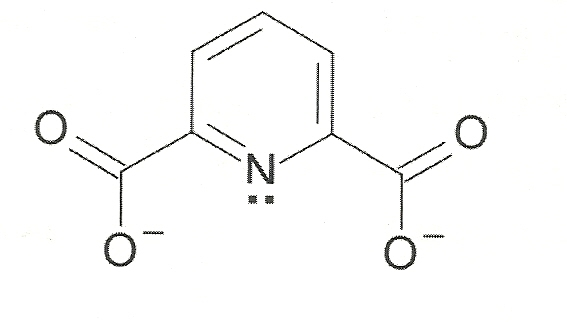
\includegraphics[scale=0.5]{./Figures/dipic.jpg}\\
  \caption{Structure of 2,6-pyridinecarboxylate (dipic)\cite{bib:lab_manual}}\label{fig:dipic}
\end{figure}

\subsection{Mechanism}
When $[dipic] >> [CA]$, that is, when $\frac{[dipic]}{[CA]} \ge 25$, then the removal of zinc is pseudo-first-order with respect to CA$\cdot$Zn because the concentration of dipic, denoted as L, does not change appreciably. Thus the formation of the inactive enzyme, apoCA, can be modeled using the following rate equation:
\begin{equation}\label{eqn:apoCA_kobs}
\frac{d[\text{apoCA}]}{dt}=k_{obs}[\text{CA$\cdot$Zn}]
\end{equation}
The pseudo-first-order rate constant, $k_{obs}$, increases as [L] increases, but levels off at sufficiently high concentrations of L. Biochemists will recognize behavior similar to Michaelis-Menten enzyme kinetics in which the enzyme, CA$\cdot$Zn, and the substrate, L, reversibly form a CA$\cdot$Zn$\cdot$L complex with association constant $K_{EML}$ (EML stands for Enzyme-Metal-Ligand):
\begin{align}\label{eqn:KEML_reaction}
\ce{CA$\cdot$Zn + L
<=>[\ce{K_{EML}}]
CA$\cdot$Zn$\cdot$L}
\end{align}
This can be modeled as follows:
\begin{equation}\label{eqn:KEML_expression}
K_{EML}=\frac{\text{[CA$\cdot$Zn$\cdot$L]}}{\text{[CA$\cdot$Zn][L]}}
\end{equation}

CA$\cdot$Zn$\cdot$L can either revert back to the original species or irreversibly convert to the inactive form of the enzyme, apoCA, and the covalently bound zinc-dipic molecule, ZnL:
\begin{align}\label{eqn:kd_reaction}
\ce{CA$\cdot$Zn$\cdot$L
->[\ce{k_{d}}]
apoCA + ZnL}
\end{align}
This yields the following differential rate law:
\begin{equation}\label{eqn:kd_expression}
\frac{d[\text{apoCA}]}{dt}=k_{d}[\text{CA$\cdot$Zn$\cdot$L}]
\end{equation}
Note the difference in assumptions between this reaction and the Michaelis-Menten model; M-M kinetics assumes the enzyme is reformed and that only the substrate is modified, while \eqref{eqn:kd_reaction} shows that both the substrate and the enzyme are permanently modified. Recall that $\text{[L]} >> \text{[CA$\cdot$Zn]}$, so [L] can be assumed to stay constant at $\text{[L]}_0$, which is substituted into a rearranged form of equation \eqref{eqn:KEML_expression},
\begin{equation}\label{eqn:KEML_expression_constant_L}
\text{[CA$\cdot$Zn$\cdot$L]}=K_{EML}\text{[CA$\cdot$Zn][L]}_0
\end{equation}

Carbonic anhydrase can exist in one of three forms: the metalloenzyme CA$\cdot$Zn, the enzyme-metal-ligand complex CA$\cdot$Zn$\cdot$L, or the inactivated enzyme apoCA. Initially, all CA is tied up in the metalloenzyme, and none exists as CA$\cdot$Zn$\cdot$L or apoCA. As the activated form of the enzyme gets bound to L and then inactivated,
\begin{equation}\label{eqn:CAZnconc}
\text{[CA$\cdot$Zn]}=\text{[CA$\cdot$Zn]}_0 - \text{[apoCA]} - \text{CA$\cdot$Zn$\cdot$L},
\end{equation}
which can be combined with equation \eqref{eqn:KEML_expression_constant_L} to yield
\begin{equation}\label{eqn:CAZnconc_EMLsub}
\text{[CA$\cdot$Zn]}=\text{[CA$\cdot$Zn]}_0 - \text{[apoCA]} - K_{EML}\text{[CA$\cdot$Zn][L]}_0
\end{equation}
and can be rearranged as follows:
\begin{equation}\label{eqn:CAZnconc_EMLsub_rearrange}
\text{[CA$\cdot$Zn]}=\frac{\text{[CA$\cdot$Zn]}_0 - \text{[apoCA]}}{1+K_{EML}\text{[L]}_0}
\end{equation}

Equations \eqref{eqn:kd_expression} and \eqref{eqn:KEML_expression_constant_L} can be combined to give
\begin{equation}\label{eqn:rate_apoCA_formation_wrt_kdkeml}
\frac{d[\text{apoCA}]}{dt}=k_{d}K_{EML}\text{[CA$\cdot$Zn][L]}_0
\end{equation}
Therefore, the rate of apoCA formation is first-order with respect to CA$\cdot$Zn. Combining equations \eqref{eqn:rate_apoCA_formation_wrt_kdkeml} and \eqref{eqn:CAZnconc_EMLsub_rearrange} yields
\begin{equation}\label{eqn:preintegration}
\frac{d[\text{apoCA}]}{dt}=k_{d}K_{EML}\text{[L]}_0\frac{\text{[CA$\cdot$Zn]}_0 - \text{[apoCA]}}{1+K_{EML}\text{[L]}_0}
\end{equation}
Rearranging and integrating,
\begin{align}\label{eqn:kdkeml_integral}
\begin{split}
\int_{[apoCA]_0}^{[apoCA]_t} \frac{d[\text{apoCA}]}{\text{[CA$\cdot$Zn]}_0 - \text{[apoCA]}_t} &= \int_0^t \frac{k_{d}K_{EML}\text{[L]}_0}{1+K_{EML}\text{[L]}_0}dt \\
&= \frac{k_{d}K_{EML}\text{[L]}_0}{1+K_{EML}\text{[L]}_0}t
\end{split}
\end{align}
The left side must be integrated using u-sub:
\begin{equation*}
u=\text{[CA$\cdot$Zn]}_0 - \text{[apoCA]}_t
\end{equation*}
\begin{equation*}
du=-d[\text{apoCA}]
\end{equation*}
To change the integral boundaries,
\begin{equation*}
u(t=0)=\text{[CA$\cdot$Zn]}_0\text{, since no inactivated enzyme has been formed}
\end{equation*}
\begin{equation*}
u(t=t)=\text{[CA$\cdot$Zn]}_0 - \text{[apoCA]}_t
\end{equation*}
Therefore,
\begin{align}\label{eqn:long_integral}
\begin{split}
\int_{[apoCA]_0}^{[apoCA]_t} \frac{d[\text{apoCA}]}{\text{[CA$\cdot$Zn]}_0 - \text{[apoCA]}_t}
&=
-\int_{\text{[CA$\cdot$Zn]}_0}^{\text{[CA$\cdot$Zn]}_0 - \text{[apoCA]}_t} \frac{du}{u} \\
&=
-ln(u) \Big|_{\text{[CA$\cdot$Zn]}_0}^{\text{[CA$\cdot$Zn]}_0 - \text{[apoCA]}_t} \\
&= -ln \left( \frac{\text{[CA$\cdot$Zn]}_0 - \text{[apoCA]}}{\text{[CA$\cdot$Zn]}_0} \right)
\end{split}
\end{align}

Combining the evaluated integrals from equations \eqref{eqn:long_integral} and \eqref{eqn:kdkeml_integral} yields
\begin{equation}\label{eqn:integrated_rate_law}
ln \left( \frac{\text{[CA$\cdot$Zn]}_0 - \text{[apoCA]}}{\text{[CA$\cdot$Zn]}_0} \right) 
=
-\frac{k_{d}K_{EML}\text{[L]}_0}{1+K_{EML}\text{[L]}_0}t 
\end{equation}
Assuming steady-state conditions for CA$\cdot$Zn$\cdot$L, that is, [CA$\cdot$Zn$\cdot$L] is always negligible, then $\frac{\text{[CA$\cdot$Zn]}_0 - \text{[apoCA]}}{\text{[CA$\cdot$Zn]}_0}$ is simply the fraction of CA$\cdot$Zn remaining after reaction time $t$ and can be referred to as $F_\text{CA$\cdot$Zn}$:
\begin{equation}\label{eqn:integrated_rate_law_frac}
ln \left( F_\text{CA$\cdot$Zn} \right)
=
-\frac{k_{d}K_{EML}\text{[L]}_0}{1+K_{EML}\text{[L]}_0}t
\end{equation}
Since $-\frac{k_{d}K_{EML}\text{[L]}_0}{1+K_{EML}\text{[L]}_0}$ is a constant for a given concentration of dipic, equation \eqref{eqn:integrated_rate_law_frac} exhibits linear behavior while the solution contains active enzyme. Therefore, a linear least squares regression procedure can be performed for measurements of $ln \left( F_\text{CA$\cdot$Zn} \right)$ over time (until those measurements level off, which indicates that all the enzyme is used up), and the slope, denoted $-k_{obs}$, will be
\begin{equation}\label{eqn:kobs_slope}
-k_{obs}
=
-\frac{k_{d}K_{EML}\text{[L]}_0}{1+K_{EML}\text{[L]}_0}
\end{equation}

Taking the reciprocal of equation \eqref{eqn:kobs_slope} yields
\begin{equation}\label{eqn:kobs_slope_reciprocal}
\begin{split}
\frac{1}{k_{obs}}
&=
\frac{1+K_{EML}\text{[L]}_0}{k_{d}K_{EML}\text{[L]}_0} \\
&= \frac{1}{k_{d}K_{EML}\text{[L]}_0} + \frac{K_{EML}\text{[L]}_0}{k_{d}K_{EML}\text{[L]}_0} \\
&= \frac{1}{k_{d}K_{EML}} \times \frac{1}{\text{[L]}_0} + \frac{1}{k_{d}}
\end{split}
\end{equation}
Again, a linear pattern is observed; measuring $k_{obs}$ at several different dipic concentrations enables one to perform a least squares regression procedure on $\frac{1}{k_{obs}}$ versus $\frac{1}{\text{[L]}_0}$ to determine the slope, $m=\frac{1}{k_{d}K_{EML}}$, and intercept, $b=\frac{1}{k_{d}}$. $k_d$ and $K_{EML}$ are thus calculated as follows:
\begin{equation}\label{eqn:calculating_kd}
k_d=\frac{1}{b}
\end{equation}
\begin{equation}\label{eqn:calculating_keml}
K_{EML}=\frac{b}{m}
\end{equation}

\subsection{Rate Measurements}
While equations \eqref{eqn:integrated_rate_law_frac} and \eqref{eqn:kobs_slope} seem to imply that the determination of $k_{obs}$ requires knowing [CA$\cdot$Zn] or [apoCA] at any point in time, in reality a plot of $f(t)$ vs $t$, where $f(t)$ is proportional to $F_\text{CA$\cdot$Zn}$, will still exhibit the same slope $-k_{obs}$. The Michaelis-Menten kinetics model states that, for sufficiently large substrate concentrations, the enzyme is fully saturated and the reaction velocity asymptotically approaches a number, $V_{max}=k_{cat}\text{[CA$\cdot$Zn]}$, where $k_{cat}$ (the ``turnover number'') is amount of substrate that can be converted to product by a single saturated enzyme molecule in a given unit of time \cite{bib:lehninger_mm}. Thus for sufficiently large concentrations of substrate, the enzyme catalytic activity fulfills the requirement of proportionality to $F_\text{CA$\cdot$Zn}$. Ideally, the determination of the enzymatic activity from $V_{max}$, that is, an \underline{enzyme assay}, can be done using a substrate which is cheap, readily available, and easily measurable. As Figure \ref{fig:pnpa_reaction} shows, carbonic anhydrase happens to hydrolyze para-nitrophenyl acetate (pNPA) to form para-nitrophenol and acetic acid:
\begin{figure}[h]
  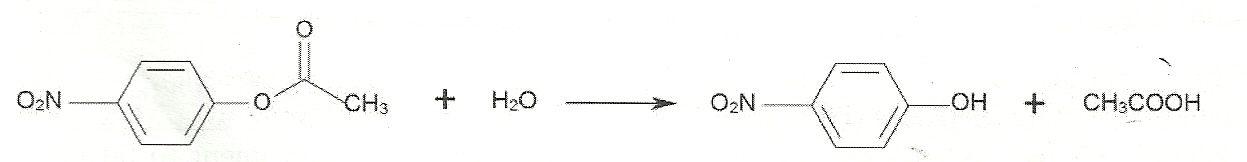
\includegraphics[width=.9\textwidth]{./Figures/pnpa_hydrolysis.jpg}\\
  \caption{Carbonic anhydrase-catalyzed hydrolysis of para-nitrophenyl acetate (pNPA) to para-nitrophenol and acetic acid \cite{bib:lab_manual}}\label{fig:pnpa_reaction}
\end{figure}

Para-nitrophenol absorbs strongly at 348nm. Recall that Beer's law states
\begin{equation}\label{eqn:beers_law}
A=\epsilon b c
\end{equation}
where $A$ is the measured absorbance at a particular wavelength, $\epsilon$ is the molar absorptivity, $b$ is the measurement path length, and $c$ is the concentration \cite{bib:quantitative_chem_anal_beer_law}. Therefore, $\frac{dA}{dt}$ is proportional to the change in para-nitrophenol (that is, the reaction velocity). Because the reaction occurs to a nontrivial extent without enzyme catalysis, a baseline correction is needed, $(\frac{dA}{dt})_{uncat}$, which can be obtained either from a solution containing only pNPA or a mixture of pNPA and apoCA (that is, after sufficient time has passed to inactivated all carbonic anhydrase before taking the assay). Thus, equation \eqref{eqn:integrated_rate_law_frac} can be implemented using $ln \left( \frac{ \frac{dA}{dt} }{ \left (\frac{dA}{dt}\right)_{uncat} } \right)$. 
\section{Procedure}
This experiment was performed using a Spectral Instruments model SI 440 spectrophotometer, which includes a CCD detector and fiber optic probe. The spectrophotometer was set to detect absorbance at 348 nm every five seconds for a total of two minutes. Device precison was set to "low," and a blank was obtained and locked. A sample of deionized water was measured to ensure absorbance stayed constant, preventing systematic errors from faulty instrumentation.

A 0.003 M aqueous pNPA solution was prepared by dissolving 25 mg solid pNPA in 1.5 mL acetone within a 250 mL Erlenmeyer flask, then slowly adding 50 mL deionized water while stirring vigorously to prevent precipitation. Assays were constructed by combining 1.7 mL deionized water, 0.3 mL HEPES buffer (0.25 M, pH 8.0), and 1.0 mL pNPA solution.

To measure the uncatalyzed assay velocity, 40 �L deionized water was added to an assay, and the absorbance was measured for two minutes. $\left( \frac{dA}{dt} \right)_{uncat}$ was found to be $3.18\times10^{-5}$.

Five dipic concentrations were tested: 0.20 M, 0.10 M, 0.05 M, 0.032 M, and 0.016 M. For each [dipic], a 500 �L solution was prepared consisting of 250 �L aqueous bovine carbonic anhydrase ($10^{-4}$ M in 0.125 M phosphate buffer, pH 7.5) and the required volumes of phosphate buffer (0.125 M, pH 7.4) and dipic (0.4 M in 0.125 M phosphate buffer, pH 7.4) needed to dilute to the specified [dipic]. In each run, the carbonic anhydrase and buffer were mixed and placed in a $25^{\circ}$C water bath to equilibrate for several minutes. Dipic was mixed just prior to starting measurements. After one minute, and then again at regular intervals over the course of one hour (or until $\frac{dA}{dt}$ measurements stopped decreasing), a 40 �L aliquot of CA/dipic solution was transferred to an assay cuvette, and a two-minute $\frac{dA}{dt}$ measurement was recorded. 
\section{Data and Results}
Five experiments were performed using a constant amount of carbonic anhydrase and varying concentrations of dipic. For each experiment, several measurements of CA-catalyzed pNPA hydrolysis velocities, $ln \left(\frac{dA}{dt}\right)_{cat}$, were taken using spectrophotometry and plotted against the CA/dipic reaction time. The results of these experiments are shown in Figure \ref{fig:kobs_results}.
\begin{figure}[h]
        \begin{subfigure}{0.5\textwidth}
                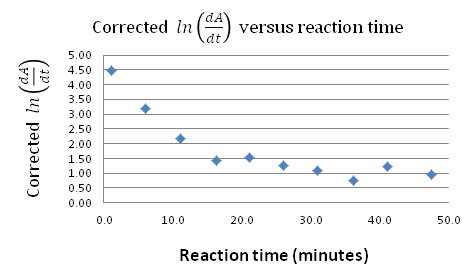
\includegraphics[width=\textwidth]{./Figures/20M_dipic_readings.png}
                \caption{0.20 M dipic}
                \label{fig:0.20M_dipic_readings}
        \end{subfigure}\begin{subfigure}{0.5\textwidth}
                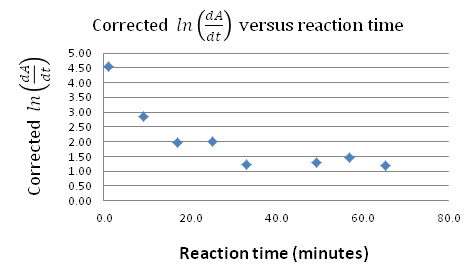
\includegraphics[width=\textwidth]{./Figures/10M_dipic_readings.png}
                \caption{0.10 M dipic}
                \label{fig:0.10M_dipic_readings}
        \end{subfigure}
        \begin{subfigure}{0.5\textwidth}
                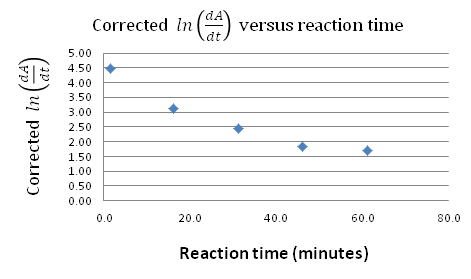
\includegraphics[width=\textwidth]{./Figures/05M_dipic_readings.png}
                \caption{0.05 M dipic}
                \label{fig:0.05M_dipic_readings}
        \end{subfigure}\begin{subfigure}{0.5\textwidth}
                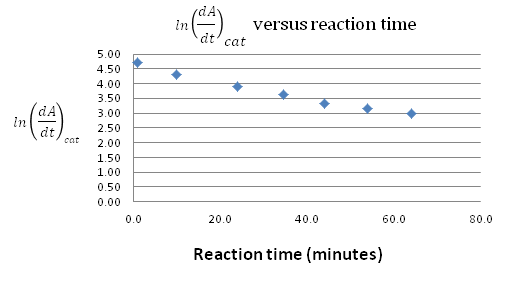
\includegraphics[width=\textwidth]{./Figures/016M_dipic_readings.png}
                \caption{0.016 M dipic}
                \label{fig:0.016M_dipic_readings}
        \end{subfigure}
        \begin{subfigure}{0.5\textwidth}
                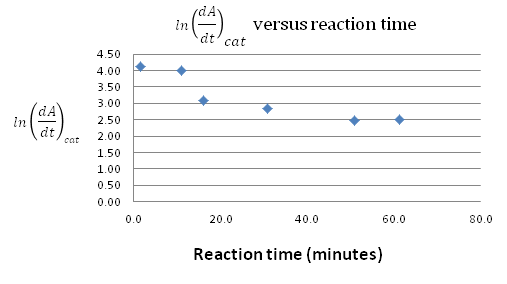
\includegraphics[width=\textwidth]{./Figures/032M_dipic_readings.png}
                \caption{0.032 M dipic}
                \label{fig:0.032M_dipic_readings}
        \end{subfigure}
        \caption{$ln \left(\frac{dA}{dt}\right)_{cat}$ measurements versus CA/dipic reaction time for various concentrations of dipic. Slopes of the descending portions of these plots were used to assign values for $k_{obs}$.}\label{fig:kobs_results}
\end{figure}

From the descending portions of the plots shown in Figure \ref{fig:kobs_results}, five values of $k_{obs}$ were calculated using the slopes determined by least squares regression. The reciprocals of $k_{obs}$ and $\text{[L]}_0$ (dipic concentration) were plotted against each other, as shown in Figure \ref{fig:kobs_vs_l}.

\begin{figure}[h]
  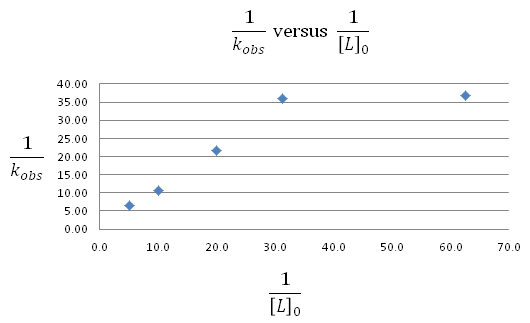
\includegraphics[scale=.5]{./Figures/kobs_vs_l.png}\\
  \caption{Plot of $\frac{1}{k_{obs}}$ versus $\frac{1}{\text{[L]}_0}$. The slope and intercept of the line passing through these points were determined by least squares regression and used to calculate $K_{EML}$ and $k_d$, demonstrated by Equations \eqref{eqn:samp_calc_keml} and \eqref{eqn:samp_calc_kd} respectively.}\label{fig:kobs_vs_l}
\end{figure}

A least squares regression procedure was performed on the data shown in Figure \ref{fig:kobs_vs_l} to retrieve values for the slope and intercept of the line passing through those points. Equations \eqref{eqn:samp_calc_keml} and \eqref{eqn:samp_calc_kd} show how these were used to calculate $K_{EML}$ and $k_d$. Table \ref{tbl:summary} lists these values and their 95\% confidence intervals, as well as accepted values reported in literature.

\begin{table}[h]
    \begin{tabular}{| l | l | l |}
    \hline
    Constant & Empirical Value & Accepted Value \\ \hline
    $K_{EML}$ & $(20\pm{18}){\ }M^{-1}$ & foobar \\ \hline
    $k_{d}$ & $(0.10\pm{0.10}){\ }mins^{-1}$ & blah \\ 
    \hline
    \end{tabular}
    \caption[Table caption text]{Values of $K_{EML}$ and $k_d$, as determined in this experiment as well as accepted values from literature}
    \label{tbl:summary}
\end{table}

%=============== Reference ===================%
\newpage
\begin{thebibliography}{9}

\bibitem{bib:lab_manual}
  Killian, B. J.
  \emph{Experiments for Physical Chemistry Laboratory},
  Summer 2014,
  Target Copy: Gainesville,
  \textbf{2014}.
  45 - 50.

\bibitem{bib:lehninger_mm}
  Nelson, D. L.; Cox, M. M.
  \emph{Lehninger Principles of Biochemistry},
  5th ed.;
  W. H. Freeman: New York,
  2008.
  195 - 200.

\bibitem{bib:quantitative_chem_anal_beer_law}
    Harris, D. C.
    \emph{Quantitative Chemical Analysis},
    7th Ed.;
    W. H. Freeman: New York,
    2006.
    381.

\end{thebibliography}

\end{document} 